\documentclass[11pt]{article}
\usepackage[margin=1in]{geometry}
\usepackage[T1]{fontenc}
\usepackage{lmodern}
\usepackage{amsmath,amssymb,amsthm}
\usepackage{graphicx}
\usepackage{hyperref}

\newtheorem{theorem}{Theorem}
\newtheorem{lemma}{Lemma}

\title{Eventually Monotone Variable-Exponent Iterated \(L_p\) Spaces}
\author{Run fa\_banach\_001, agent\_lane\_13}
\date{2026-06-19}

\begin{document}
\maketitle

\section*{Status}

This is a \texttt{partial\_result\_likely\_valid} packet for the variable
exponent problem in Yanqi Qiu, \emph{On the UMD constants for a class of
iterated \(L_p(L_q)\) spaces}, arXiv:1112.0739.  The result gives a positive
answer for eventually monotone exponent sequences.  It is not a full
characterization.

\section*{Source Problem}

Qiu defines, for \(1<p_i<\infty\),
\[
  X[(p_i)] = \lim_{\longrightarrow} L_{p_n}\cdots L_{p_2}L_{p_1},
  \qquad
  Z[(p_i)] = \lim_{\longrightarrow} L_{p_1}L_{p_2}\cdots L_{p_n},
\]
and asks:
\[
  \text{Under which condition is } X[(p_i)] \text{ or } Z[(p_i)]
  \text{ in the UMD class?}
\]
The paper records necessary conditions: the exponents must remain in a compact
subinterval of \((1,\infty)\), must have a unique cluster point, and must pass
the product obstruction
\[
  \prod_i c(p_i,p_{i+1}) < \infty.
\]
It then says that, intuitively, sufficiently fast convergence \(p_i\to p\)
should imply the UMD property.

\begin{center}

\includegraphics[width=0.92\linewidth]{figures/open_problem_crop.png}
\end{center}

\section*{Idea of the Proof}

Qiu's Remark~5.7 contains a finite-dimensional monotonicity observation: a
consecutive monotone block in a finite mixed-norm tower may be compressed to
its two endpoints without changing the \(UMD_s\) constant.  Therefore, if the
tail of \((p_i)\) is monotone, the whole tail \(p_N,\ldots,p_n\) contributes
no more than the two exponents \(p_N\) and \(p_n\) at level \(n\).  Since
\(p_n\) stays inside one compact interval and all other exponents left after
compression are fixed, the finite-level \(UMD_s\) constants are uniformly
bounded.  Uniform finite-level bounds pass to the inductive limit.

\begin{center}
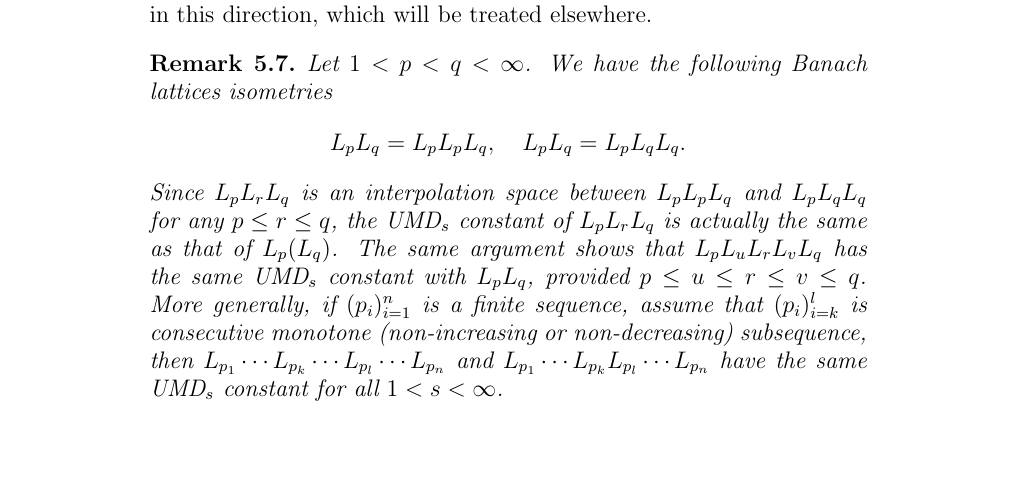
\includegraphics[width=0.92\linewidth]{figures/monotone_remark_crop.png}
\end{center}

\section*{A Standard Stability Lemma}

\begin{lemma}
\label{lem:compact-stability}
Fix \(1<s<\infty\) and a compact interval \(I=[a,b]\subset(1,\infty)\).
There is a constant \(K=K(I,s)\) such that
\[
  C_s(L_r(Y)) \le K\, C_s(Y)
\]
for every \(r\in I\) and every UMD Banach space \(Y\), where \(C_s\) denotes
the \(UMD_s\) martingale transform constant.
\end{lemma}

\begin{proof}
This is the usual vector-valued \(L_r\)-stability of the UMD property, with
constants locally bounded for \(r\) in compact subintervals of
\((1,\infty)\).  Equivalently, one may combine the standard independence of
the UMD exponent, used in Qiu's equation~(10), with the identity
\(C_r(L_r(Y))=C_r(Y)\).  The resulting constants are bounded uniformly for
\(r\in I\).
\end{proof}

\section*{Partial Theorem}

\begin{theorem}
\label{thm:eventually-monotone}
Let \((p_i)_{i\ge 1}\) satisfy
\[
  1<a\le p_i\le b<\infty
\]
for all \(i\).  Suppose that \((p_i)\) is monotone from some index \(N\)
onward.  Then both inductive limits \(X[(p_i)]\) and \(Z[(p_i)]\), in Qiu's
notation, are UMD.
\end{theorem}

\begin{proof}
Fix \(1<s<\infty\).  It is enough to show that the \(UMD_s\) constants of the
finite levels are bounded uniformly in the level.

Consider first
\[
  Z_n=L_{p_1}L_{p_2}\cdots L_{p_n}.
\]
For \(n\ge N\), the block \(p_N,p_{N+1},\ldots,p_n\) is consecutive and
monotone.  By Qiu's Remark~5.7, deleting the interior of this block does not
change the \(UMD_s\) constant.  Hence
\[
  C_s(Z_n)
  =
  C_s\bigl(L_{p_1}\cdots L_{p_N}L_{p_n}\bigr)
  \qquad (n\ge N).
\]
The right-hand side contains only the fixed layers
\(p_1,\ldots,p_N\) and one variable layer \(p_n\in[a,b]\).  Applying
Lemma~\ref{lem:compact-stability} a finite number of times gives
\[
  \sup_{n\ge N} C_s(Z_n) < \infty.
\]
The finitely many levels \(n<N\) do not affect boundedness.

For
\[
  X_n=L_{p_n}L_{p_{n-1}}\cdots L_{p_1},
\]
the reversed tail \(p_n,p_{n-1},\ldots,p_N\) is again consecutive and
monotone.  Qiu's same remark gives
\[
  C_s(X_n)
  =
  C_s\bigl(L_{p_n}L_{p_N}L_{p_{N-1}}\cdots L_{p_1}\bigr)
  \qquad (n\ge N).
\]
Again only one exponent, \(p_n\), varies in the compact interval \([a,b]\),
while all other layers are fixed.  Lemma~\ref{lem:compact-stability} yields
\[
  \sup_{n\ge N} C_s(X_n) < \infty.
\]

Finally, the inductive limits are the closures of increasing unions of the
finite levels.  Any finite martingale transform test with values in the dense
algebraic union takes its values in some finite level, where the same uniform
constant applies.  A density argument passes the inequality to the completed
inductive limit.  Thus both \(X[(p_i)]\) and \(Z[(p_i)]\) are UMD.
\end{proof}

\section*{Limitations}

The theorem does not characterize all exponent sequences.  It does not settle
oscillatory sequences with infinitely many local extrema, nor does it prove
that Qiu's necessary product condition \(\prod_i c(p_i,p_{i+1})<\infty\) is
sufficient.  It also does not compute the constants \(c(p,q)\), which Qiu
explicitly notes are unknown in general.

\section*{Search and Novelty Check}

The lane-13 queue selected arXiv:1112.0739.  Cheap run indexes were searched
for the arXiv id, title, \(UMD\) constants, \(X[(p_i)]\), \(Z[(p_i)]\), and
the product condition; no duplicate packet or attempt was found.  Local source
search found the exact variable-exponent problem only in arXiv:1112.0739.
Targeted web searches for exact phrases including
\texttt{Under which condition is X[(p\_i)]}, \texttt{Z[(p\_i)] UMD}, and
\texttt{prod\_i c(p\_i,p\_\{i+1\})} found no later exact answer beyond the
source paper.  This packet should therefore be read as a source-derived
partial theorem, not as a known later-literature resolution.

\section*{Human Review Recommendation}

The main point to check is the use of Qiu's Remark~5.7 for the reversed
finite towers defining \(X_n\).  Since reversing an eventually monotone block
keeps it monotone, the same deletion statement applies, but this is the one
step where notation and tower order should be verified against the source.

\begin{thebibliography}{9}
\bibitem{Qiu}
Y.~Qiu,
\emph{On the UMD constants for a class of iterated \(L_p(L_q)\) spaces},
arXiv:1112.0739.
\end{thebibliography}

\end{document}
